\documentclass[../main.tex]{subfiles}
\graphicspath{{\subfix{../../images/}}}
\begin{document}


 
 1. System Identification: learning a transition function $p(y_t|x_t, u_t)$
    - How do you learn the unknown observation model from data?

1. Policy Optimization
    - Once dynamics are learned (or at least stable?), how do we form a policy that is generalizable to new tasks under these dynamics?
    - This is the control problem.

It's safe to assume that these processes are happening in parallel. Because we have complete and arbitrary control over the observation mapping, we can ask the subject to interact through a  dynamic that is intuitive (informative prior) or unintuitive (uninformative or inhibitive prior). Each scenario, we hypothesize, will elicit different strategies for learning and control.






\section{Performance and its Potential Correlates}




\begin{figure}
    \phantomsection\label{fig:hit_fraction}
    \centering
    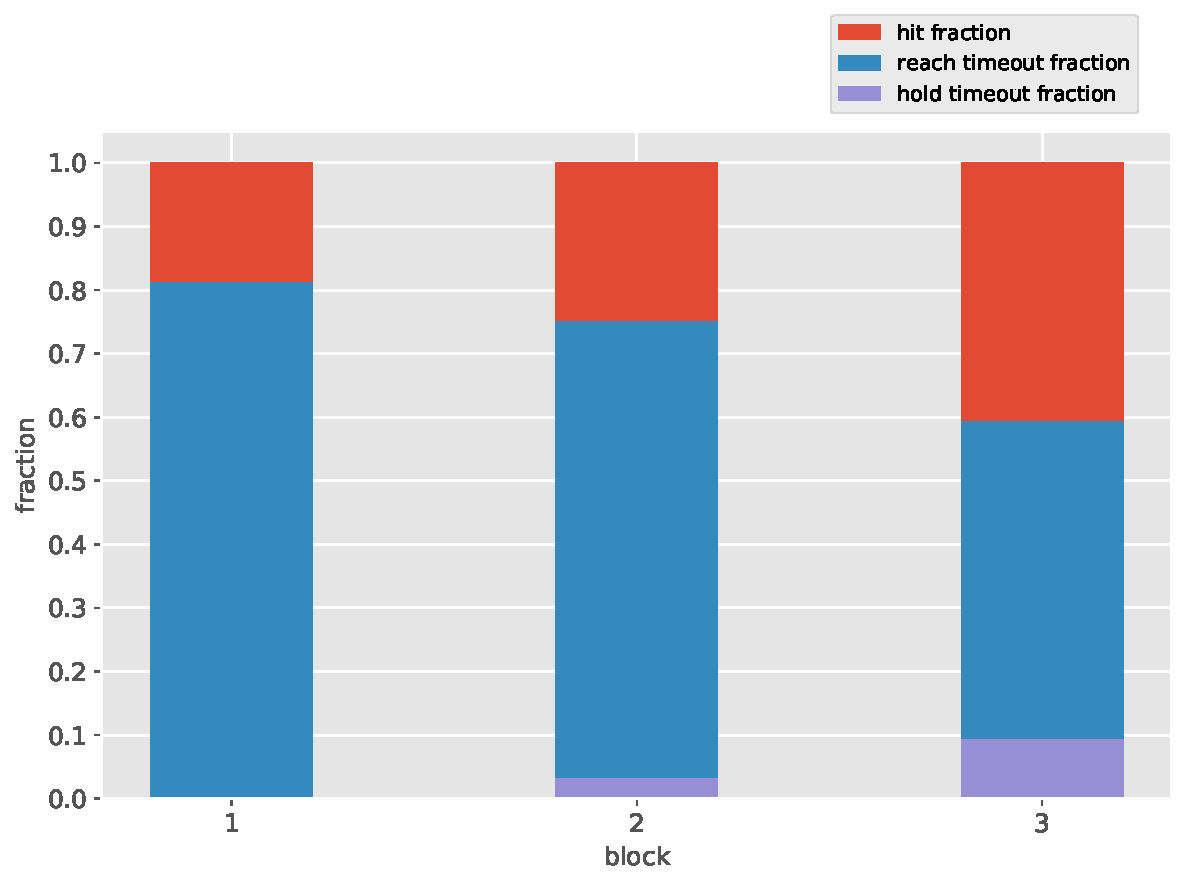
\includegraphics[width=0.2\textwidth]{images/data_analysis/center_hold/hit_fraction.pdf}
    \caption{Fractions of trial outcome types for each block of the center-hold, reach-out task. Hit fraction increases on each trial, suggesting the beginnings of task learning. Hold timeout failure increases over trials as well, perhaps suggesting increased baseline excitation of muscles during the hold period. Part of learning to activate certain muscle modes is learning to inhibit others.}\label{fig:hit_fraction}
    \end{figure}
    


In this task, the subject's first goal is to interact through the mapping $M$ and learn the consequences of various motor activations. That is, they must internalize a model of the virtual environment, what might be called a system identification problem. Subjects must collect data containing motor outputs and their sensory consequences. To do this, they must explore the space of activity. We predict that over trials, subjects' EMG activities over channels will become more varied as they attempt new movement patterns to achieve their twin goals of learning to move in this new environment and reaching the target. Running PCA on each individual trial's EMG time series, we hypothesize that initially we will see multiple components share signal variance as subjects explore. Eventually, we would expect to see a decrease in this measure of movement complexity a subjects hone their reaching skill. Trial-level PCA component variance fractions are shown in \Cref{fig:PCA_trial_variance}. We find an initial decrease in the top component's variance fraction, though we expect many more trials will be needed to see skill acquisition in the form of a dominant movement mode per trial.

\begin{figure}
\phantomsection\label{fig:PCA_trial_variance}
\centering
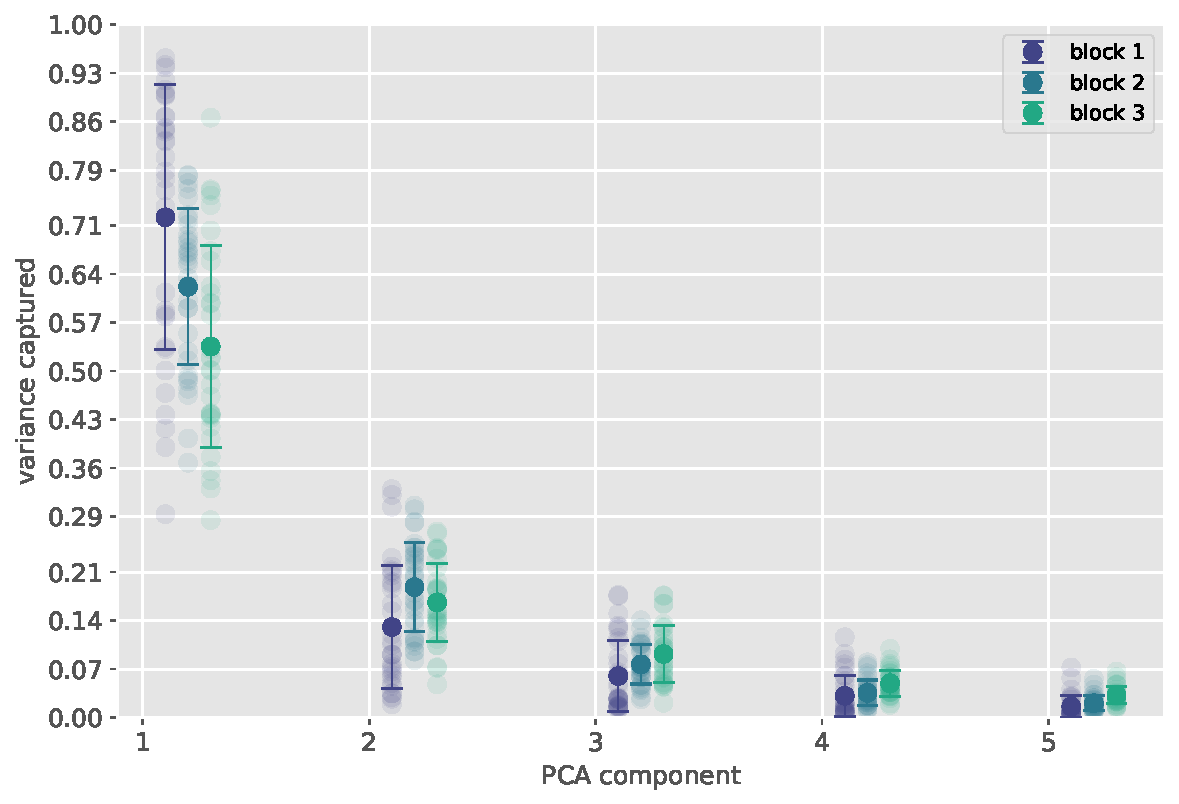
\includegraphics[width=0.2\textwidth]{images/data_analysis/center_hold/PCA_trial_variance.pdf}
\caption{Fraction of variance captured by the top five principle components when PCA is run on the EMG time series' of individual trials of the center-hold, reach-out task. Error bars are standard deviation. Over blocks, we see a slight decrease in the mean of the top component's variance fraction, though with high variance. This may suggest greater exploration within-trial, as less variance is captured by a single component over blocks, though it could reflect more varied dynamics across trials as the subject discovers new, task-relevant activations.}\label{fig:PCA_trial_variance}
\end{figure}

We might model this task as the subject selecting an EMG signal $x$ which minimizes the distance between a target position $b$ and the projection of the EMG signal through the mapping $M$ as well as minimizes the norm of $x$ in order to conserve metabolic energy. This optimization can be written as a regularized least squares problem:

\begin{align}
  \min_x\frac{1}{2}||Mx - b||^2_2 + \frac{\lambda}{2}||x||_2^2.
\end{align}

This problem is known to have a unique minimum for $\lambda>0$ which is an approximation $Mx\approx b$ regardless of the shape or rank of $M$. This implies that the subject, if they are biophysically capable to do so, will learn distinct motor outputs for each target rather than reusing modes for multiple targets with different activation levels. That is the subject will, over time, learn to fractionate their muscle output to reach their goal in order to minimize effort. For instance, to reach the the target at position $(1,0)$ in Cartesian coordinates, the subject could activate a bespoke activity mode and activate a combination of two or more modes for targets at $\pm45^\circ$ from this central target. If this is the case, the model predicts that the dimensionality of the EMG signal will increase over the course of training as the subject learns to construct bespoke activity modes for each target.

In \Cref{fig:PCA_concat_variance} we compute PCA on the concatenation of all trials within blocks for which we predict an increase in the number of dominant EMG modes as subjects learn multiple movements to reach individual targets. We expect subjects to, over time, develop some number of bespoke movement modes to activate independently and as a composition to reach each target. We find a suggestion of this idea in the data with our basic PCA analysis. More trials, session, and subjects will be required to explore this idea, and we are investigating probabilistic measures of signal complexity such as entropy to formalize this hypothesis. One direction might be to further define this task a regularized regression with different regularization terms chosen normatively for different sections of the learning and control process, and fitting data to these predictions. For instance, early in training subjects may not optimize for target accuracy as much as for signal sparsity, whereas later in learning subjects may optimize for target accuracy and output signal magnitude.

\begin{figure}
\phantomsection\label{fig:PCA_concat_variance}
\centering
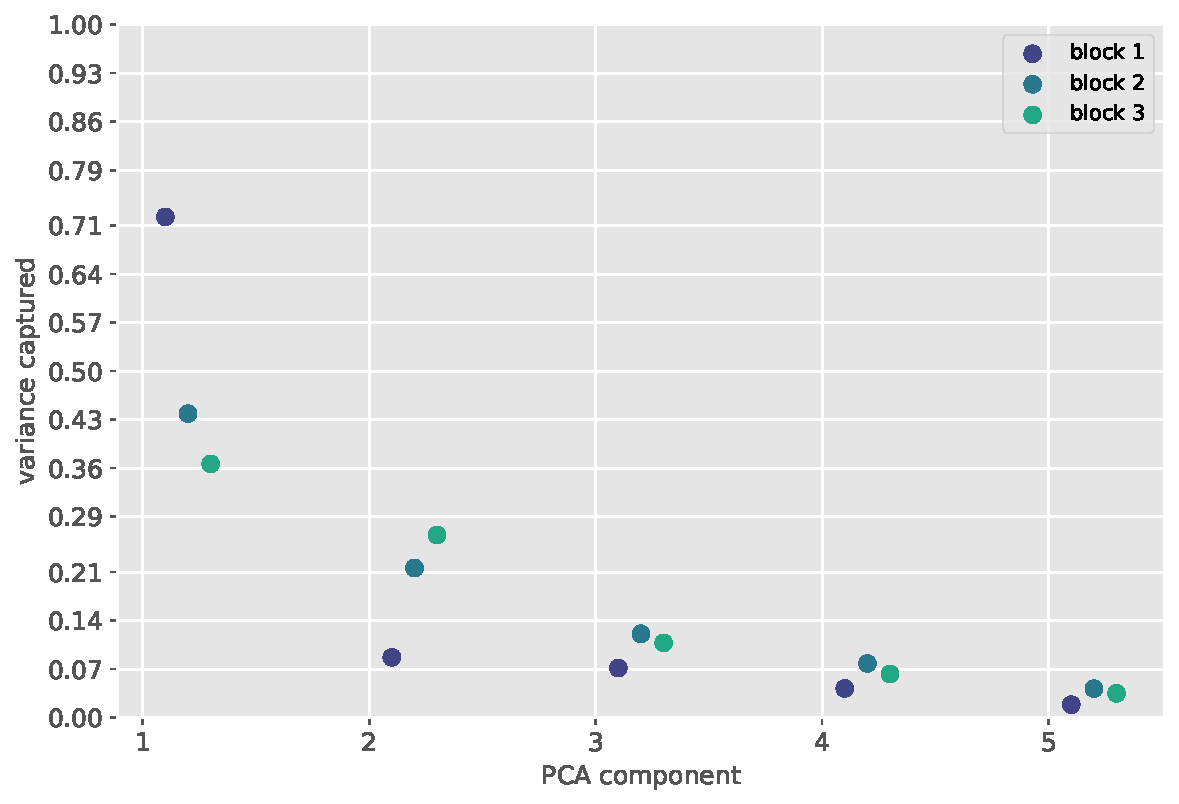
\includegraphics[width=0.2\textwidth]{images/data_analysis/center_hold/PCA_concat_variance.pdf}
\caption{Fraction of variance captured by PCA computed on concatenated EMG time series concatenated over trials. Over blocks, we see variance shifting from the top component to other components. We hypothesize that across learning we would see the development of bespoke modes used in combination to reach individual targets. This would predict an increase in the complexity of the EMG time series over learning. Here we see suggestions of this prediction.}\label{fig:PCA_concat_variance}
\end{figure}


We first asked whether PCA applied to each individual trial would extract a single, high-variance component reflecting the dimensionality of the behavior. Since each finger movement is intuitively one dimensional, we predict that PCA would find a single high-variance component when run on each individual trial. As shown in \Cref{fig:PCA_variances}, this is generally the case, though there are some outlier trials. After inspecting these outlier trials, it is likely that the subject moved multiple fingers in these trials counter to the experimenter's instruction.

\begin{figure}
\phantomsection\label{fig:PCA_variances}
\centering
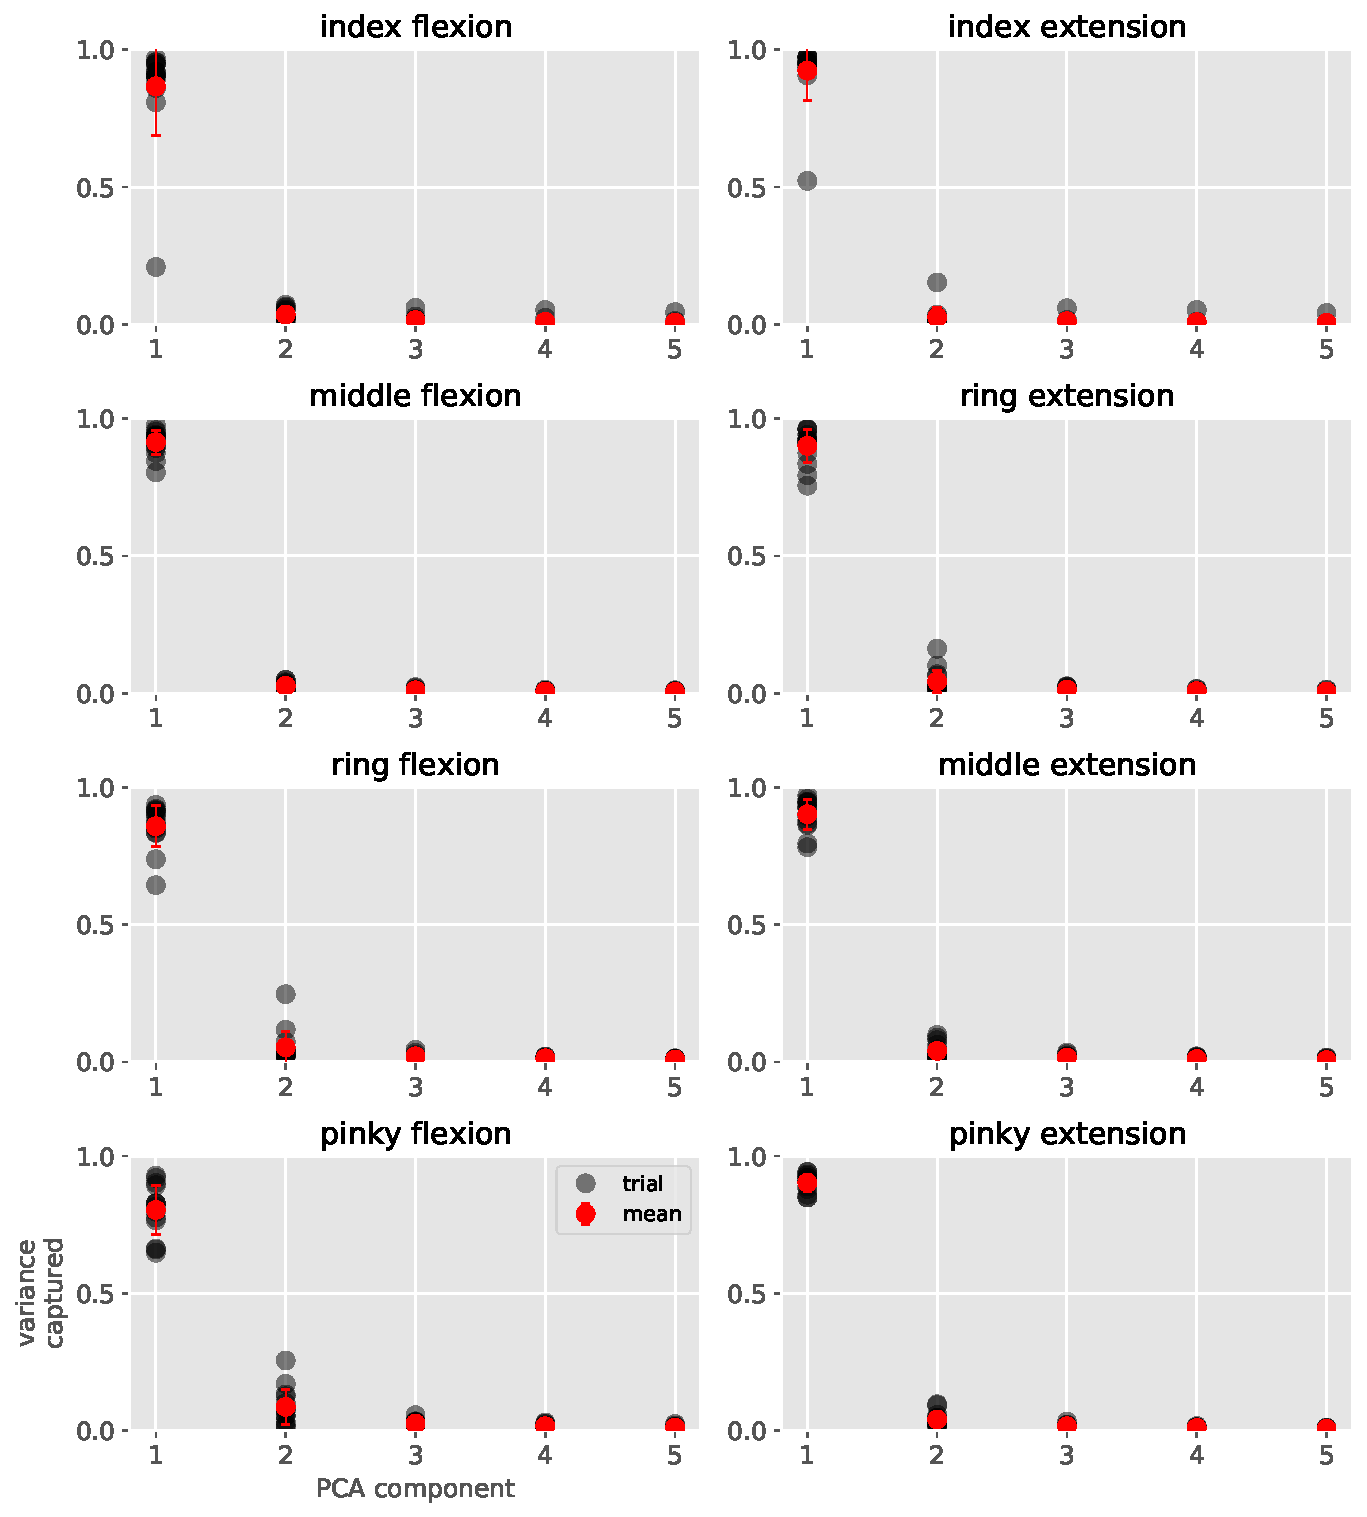
\includegraphics[width=0.2\textwidth]{images/data_analysis/fingers/PCA_variances.pdf}
\caption{Fraction of variance captured by the top 5 principle components for trials of single finger extensions and flexions. PCs were computed for individual trials. Trials were recorded from one subject for 10s each trial with finger movement frequency approximately 1Hz. Three blocks each with one trial per finger movement were recorded per day for 5 days for a total of 15 trials per finger. Electrodes were not removed between blocks but were removed between days. Each trial displays a single high-variance PC component.}\label{fig:PCA_variances}
\end{figure}

We next asked, since each trial appeared to be dominated by a single principle component, whether this top component was stable across trials and across days. If the top component is stable, it implies that the recording apparatus is robust to electrode movement between sessions. The top components for each movement after running PCA on each trial are shown in \Cref{fig:PCA_components}. While it is not typical to run PCA on individual trials, for the purpose of visually inspecting the PCA weights over EMG channels it is used here.

\begin{figure}
\phantomsection\label{fig:PCA_components}
\centering
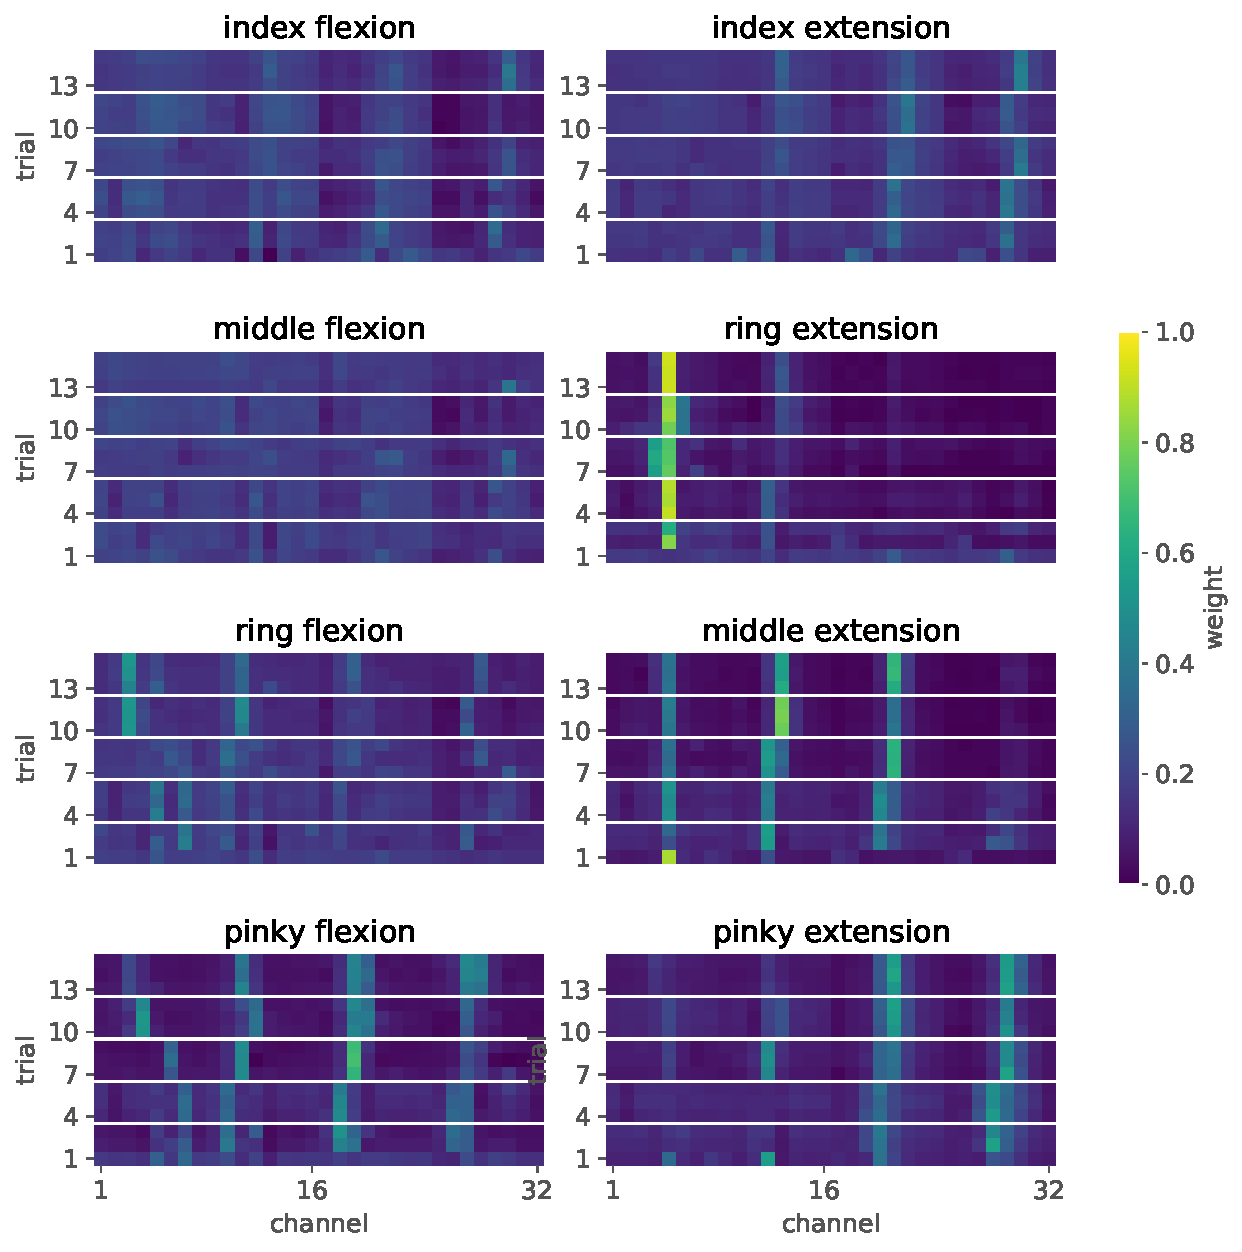
\includegraphics[width=0.2\textwidth]{images/data_analysis/fingers/PCA_components.pdf}
\caption{The top principle component from each single finger movement trials plotted as weights across channels. PCA was computed for each trial individually. White horizontal lines show breaks between days when electrodes were removed and reapplied. Each trial's top component is relatively stable across trials and across days, though there is drift and dropout of weights. Measures to increase cross-session stability are discussed in the main text. Movements appear to vary between strong localization on single channels and broad activation across channels.}\label{fig:PCA_components}
\end{figure}

The results here suggest that, at least up to linear decompositions, the features of low-contraction movements is relatively robust across sessions. As discussed in {section:next\_steps}, we will construct more reliable means to place electrodes on subjects' forearms to further increase repeatability. Another aspect of these results is our assumption subjects are producing the same contraction each time they move their finger, and at the same contraction level. That is, we assume they are recruiting the same motor units each movement. This may not be the case, and constructing new analyses which infer motor unit activations may be useful to mitigate this issue.






\begin{figure}
\centering
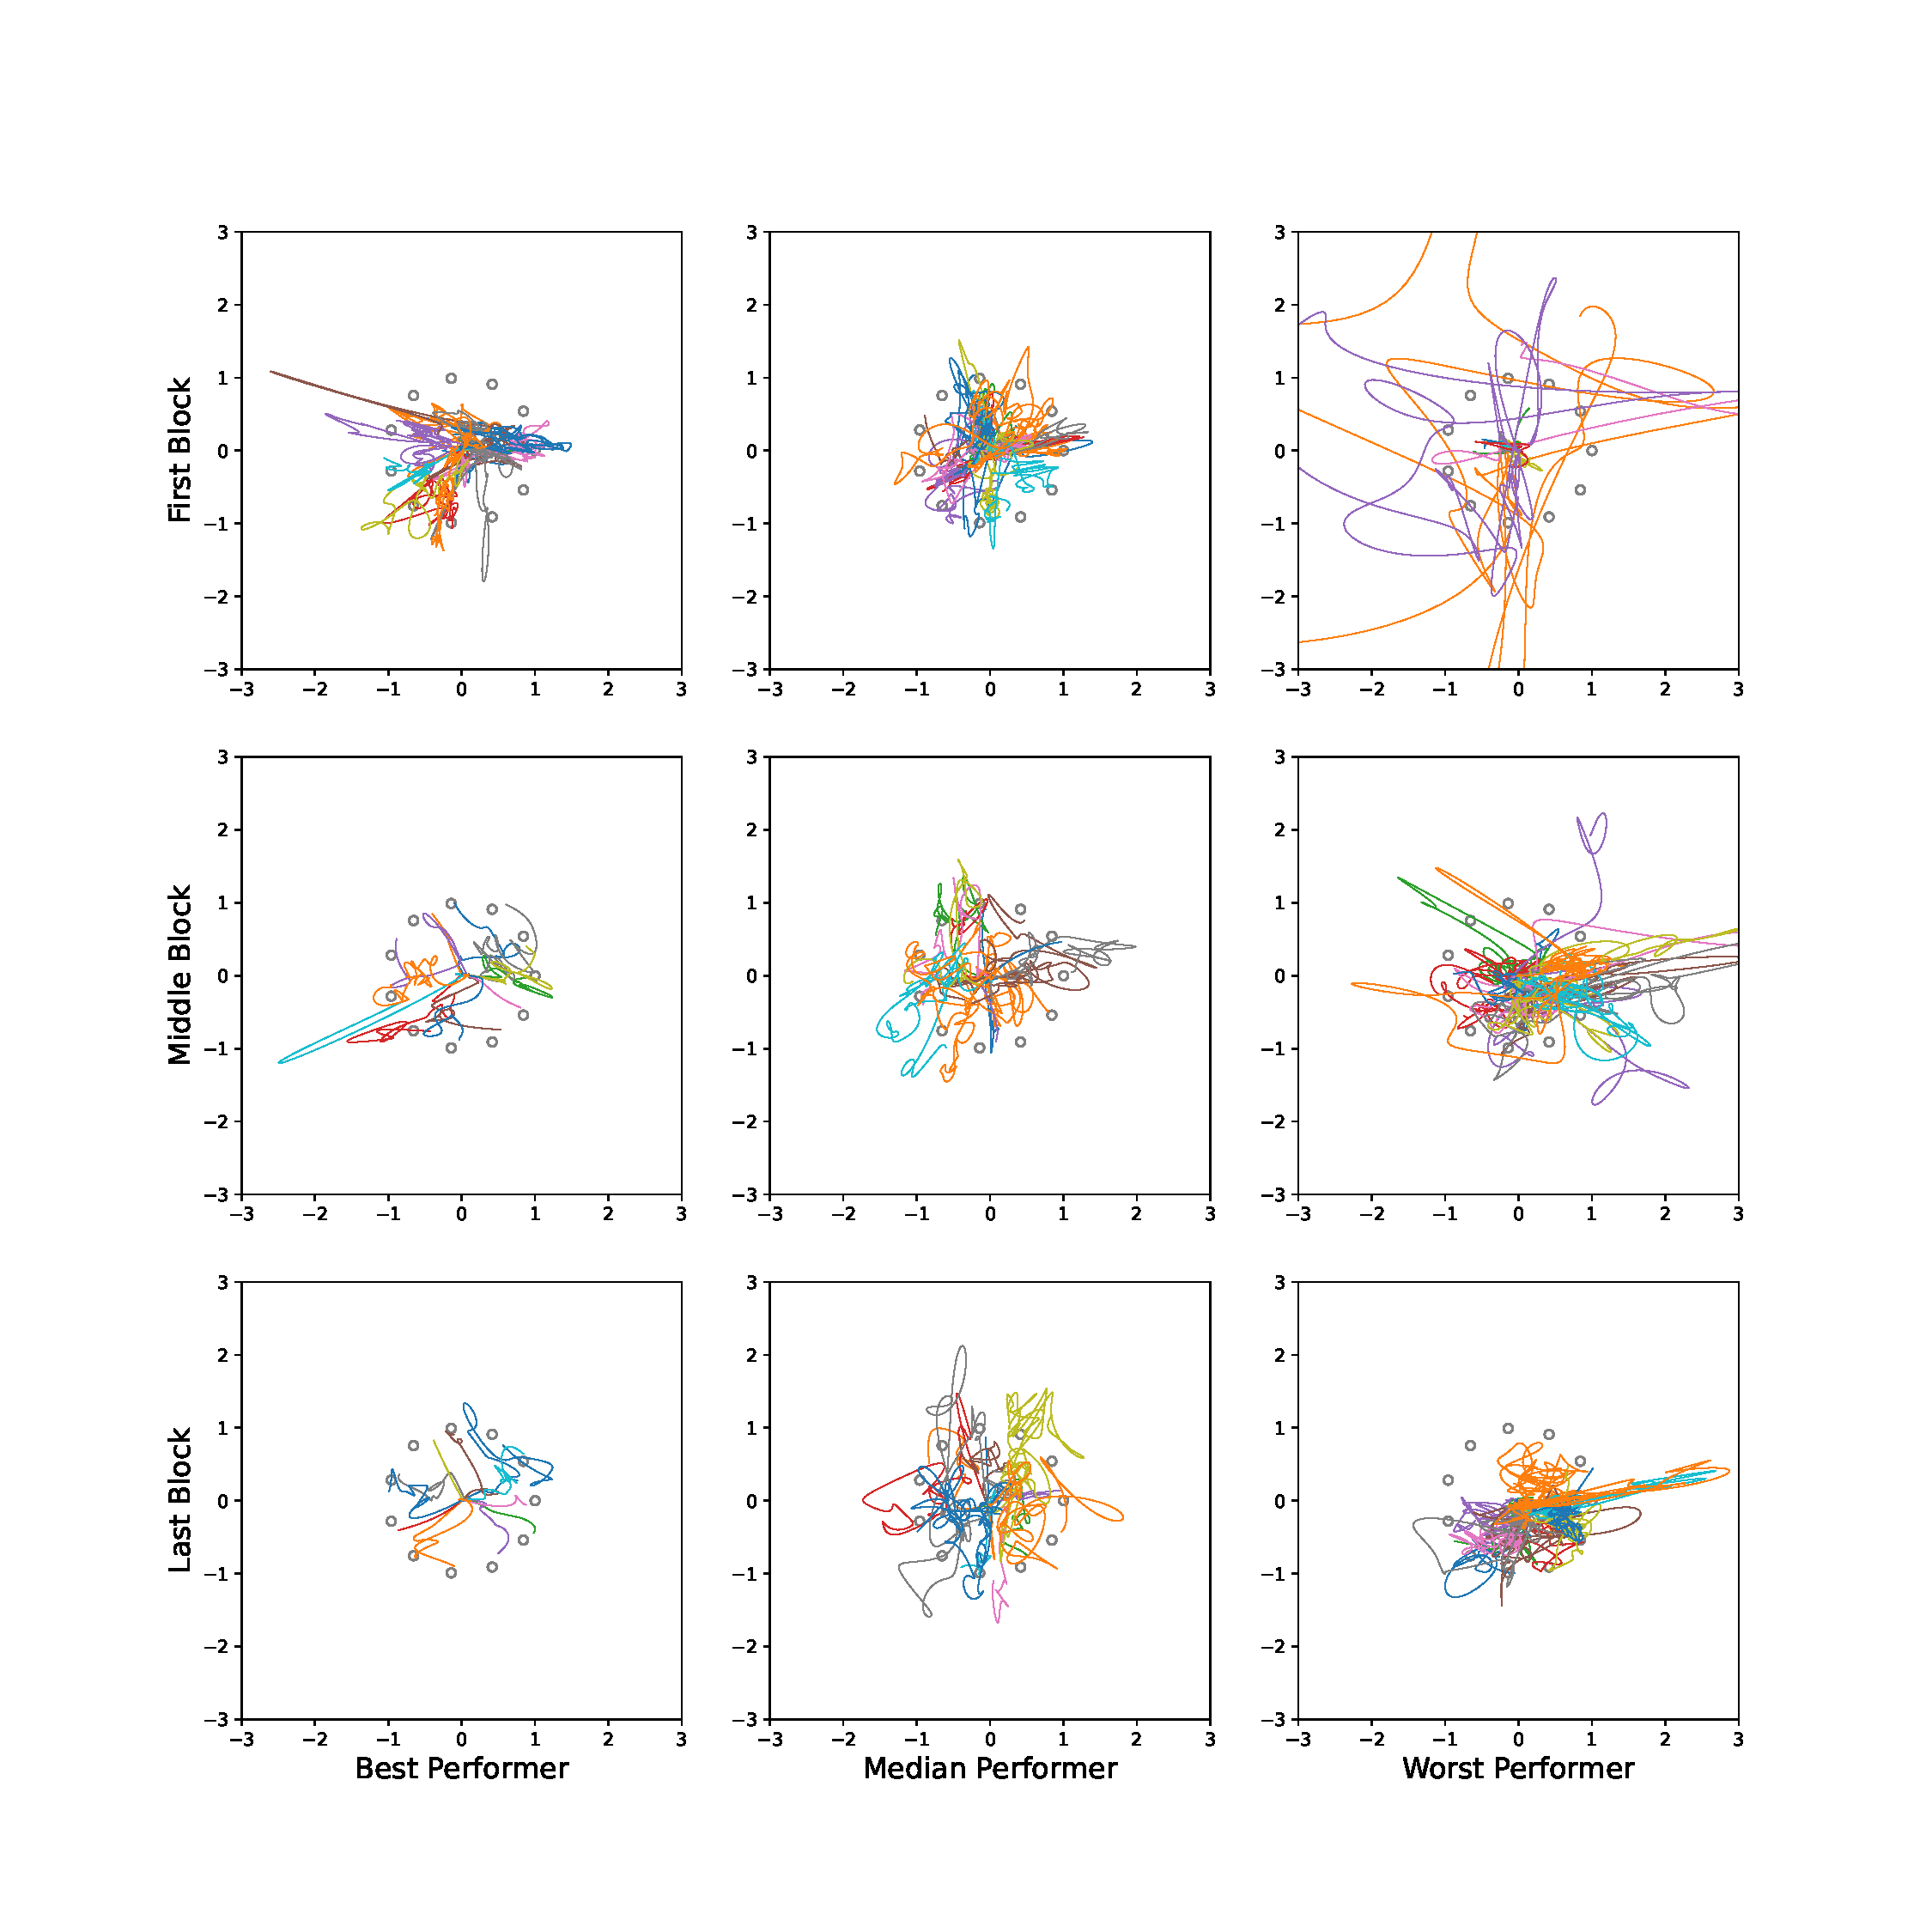
\includegraphics[width=\textwidth]{analysis/behavior.pdf}
\caption{Example task behavior. Behavioral trajectories from the
``center hold, reach out'' task. This task required subject to maintain
their cursor in the center of the frame by refraining from any muscle
activity in the recorded forearm for 2s. After this initial period, one
of 12 targets appeared on-screen (shown here as grey circles). The
subject attempted to activate their forearm muscle activity to ``reach''    
to each target. Moving their cursor to the target resulted in a ``Hit''.
The cursor was allowed to exit the ``screen'' spanning {[}-2,2{]} as
plotted here, becoming invisible to the subject. Each plot shows cursor
trajectories from a single block of 12 unique targets, each trial a
different color. Each column of three plots is a single subject, from
left to right: the subject with the most, median, and least ``Hits'
across all trials of the task. Each row shows one block of 12 trials,
from top to bottom: the first block, the halfway point, and the last
block.}\label{fig:behavior}
\end{figure}

\begin{figure}
\centering
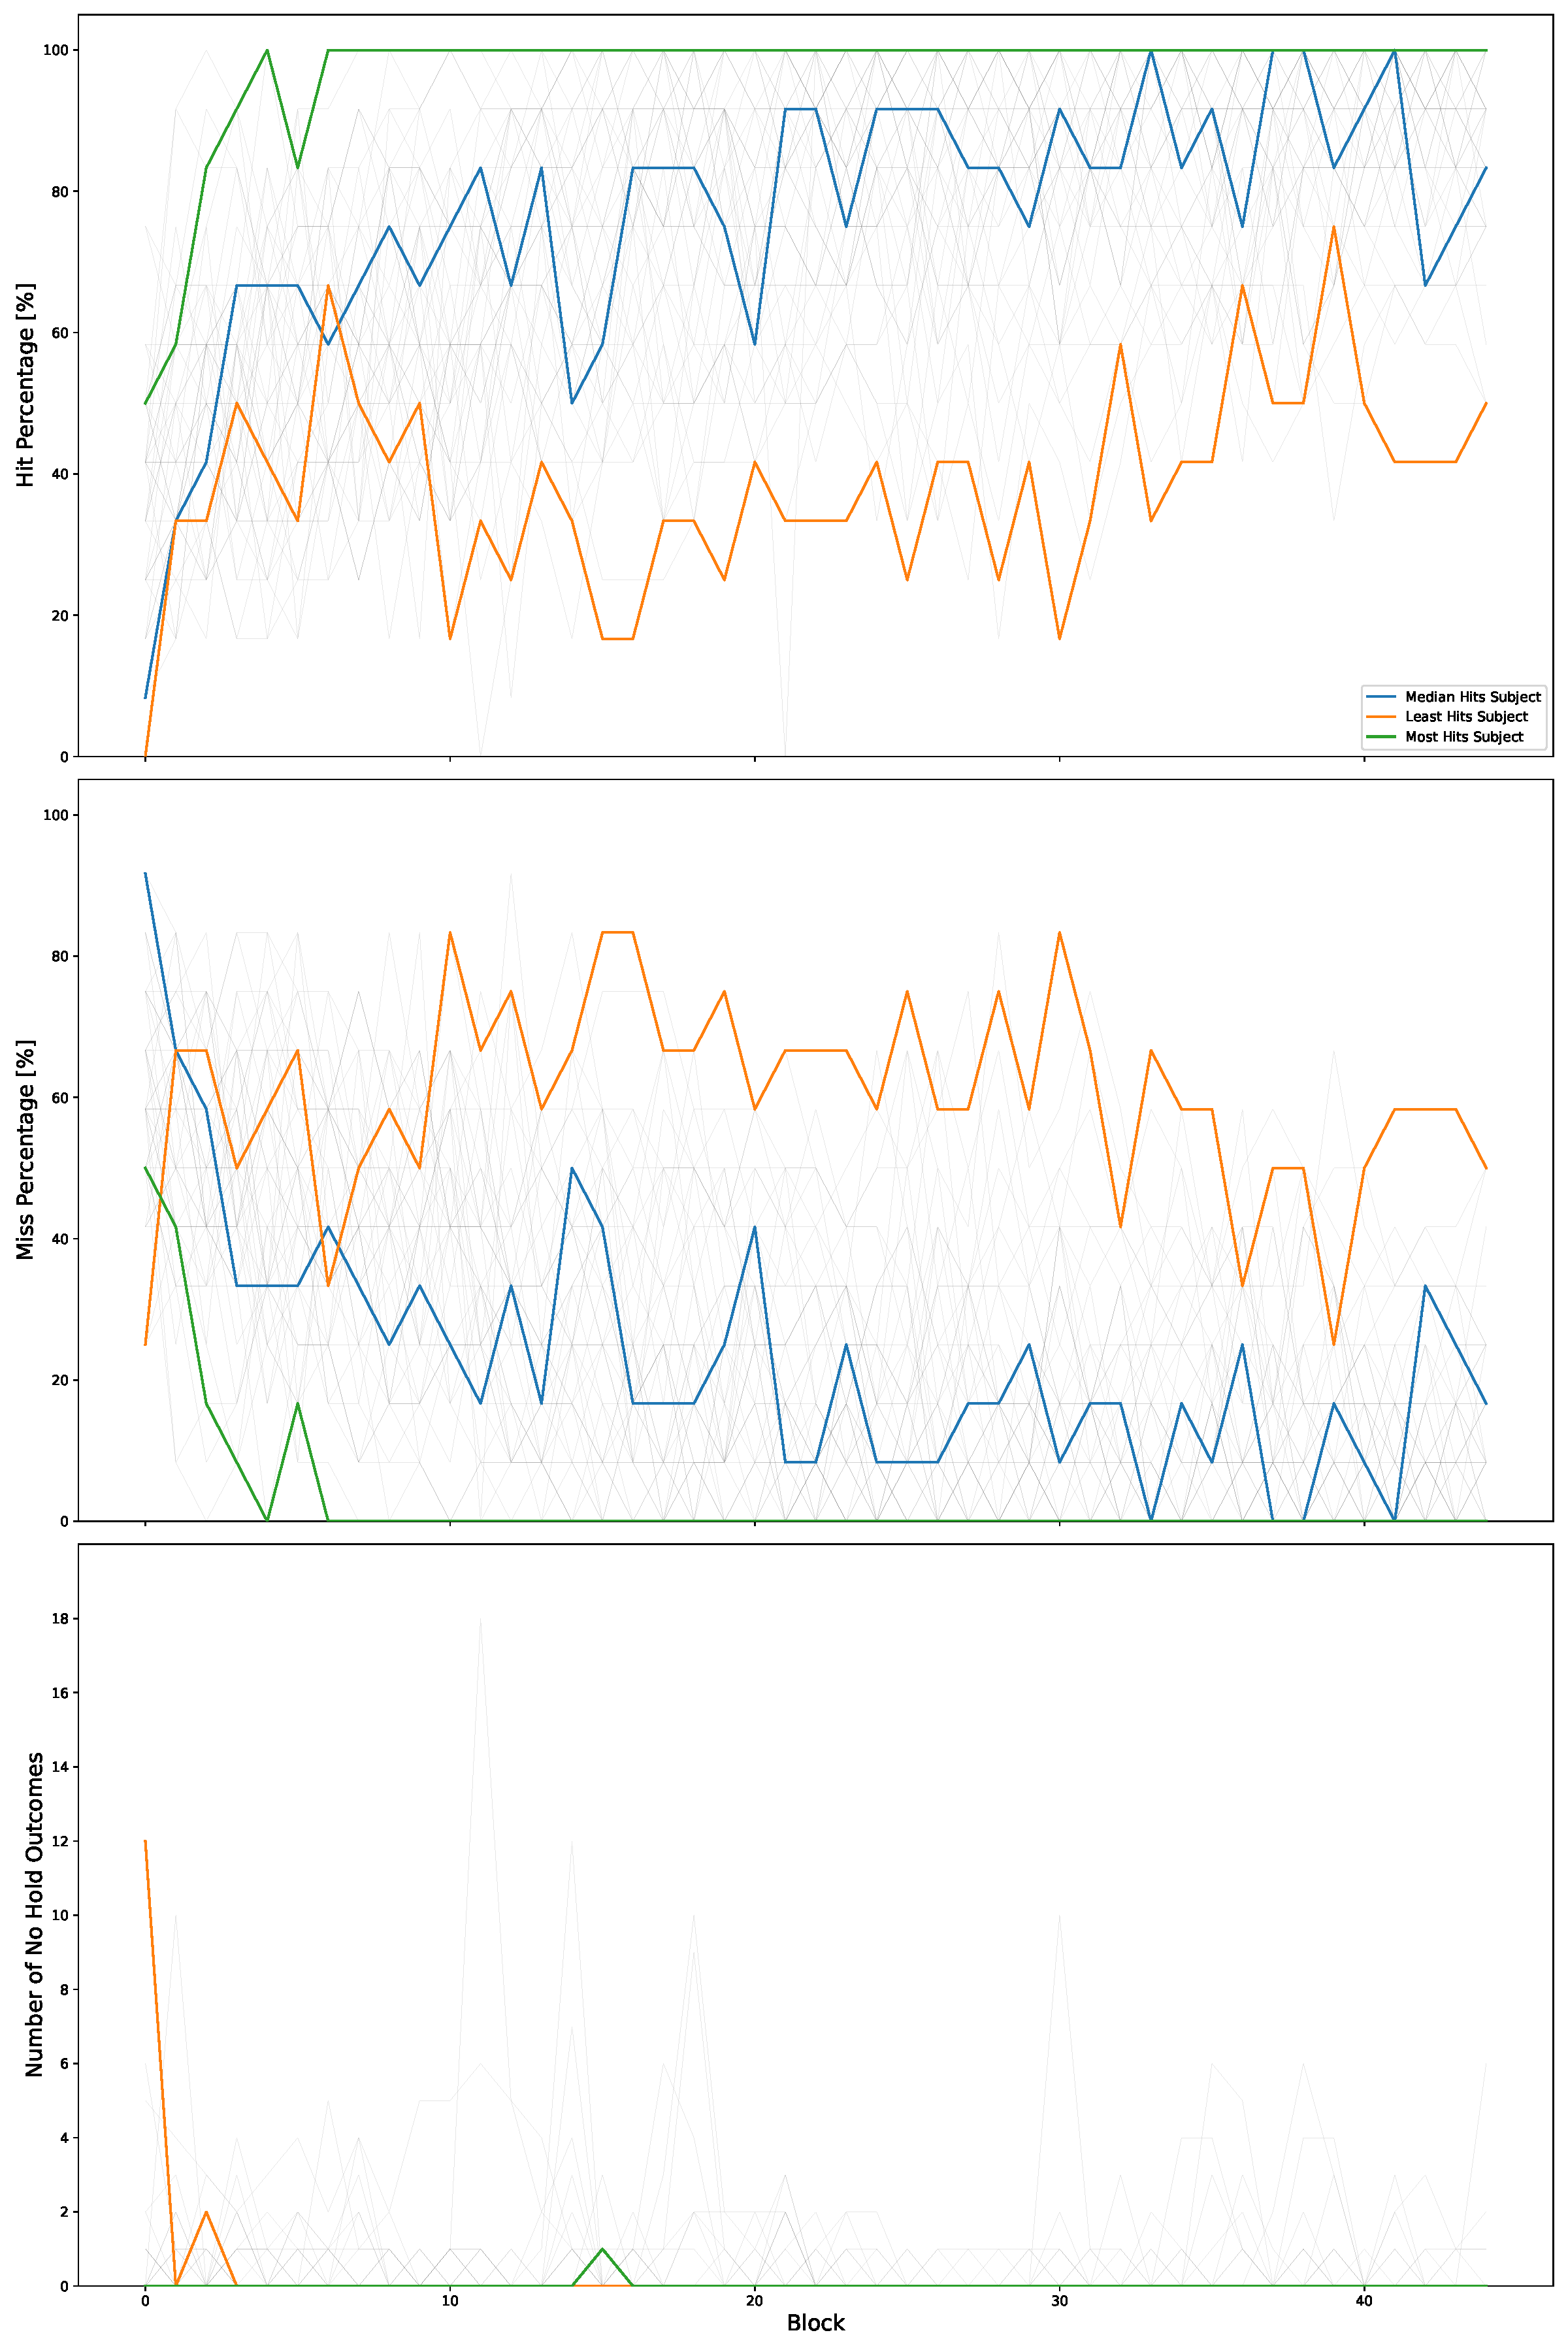
\includegraphics[width=\textwidth]{analysis/outcomes.pdf}
\caption{Task outcomes over blocks. Outcomes across all 45 blocks of 12
trials (targets) in the ``center hold, reach out'' task. Subjects with
the most, median, and least hits are shown in green, blue, and orange
respectively. All ofther subjects are show in gray. From top to bottom:
The percentage of ``Hits'' within each block, the percentage of
``Misses'' (timeouts), and ``No Holds'' (subject unable to quiet forearm
muscle activity initially).}\label{fig:outcomes}
\end{figure}

\begin{figure}
\centering
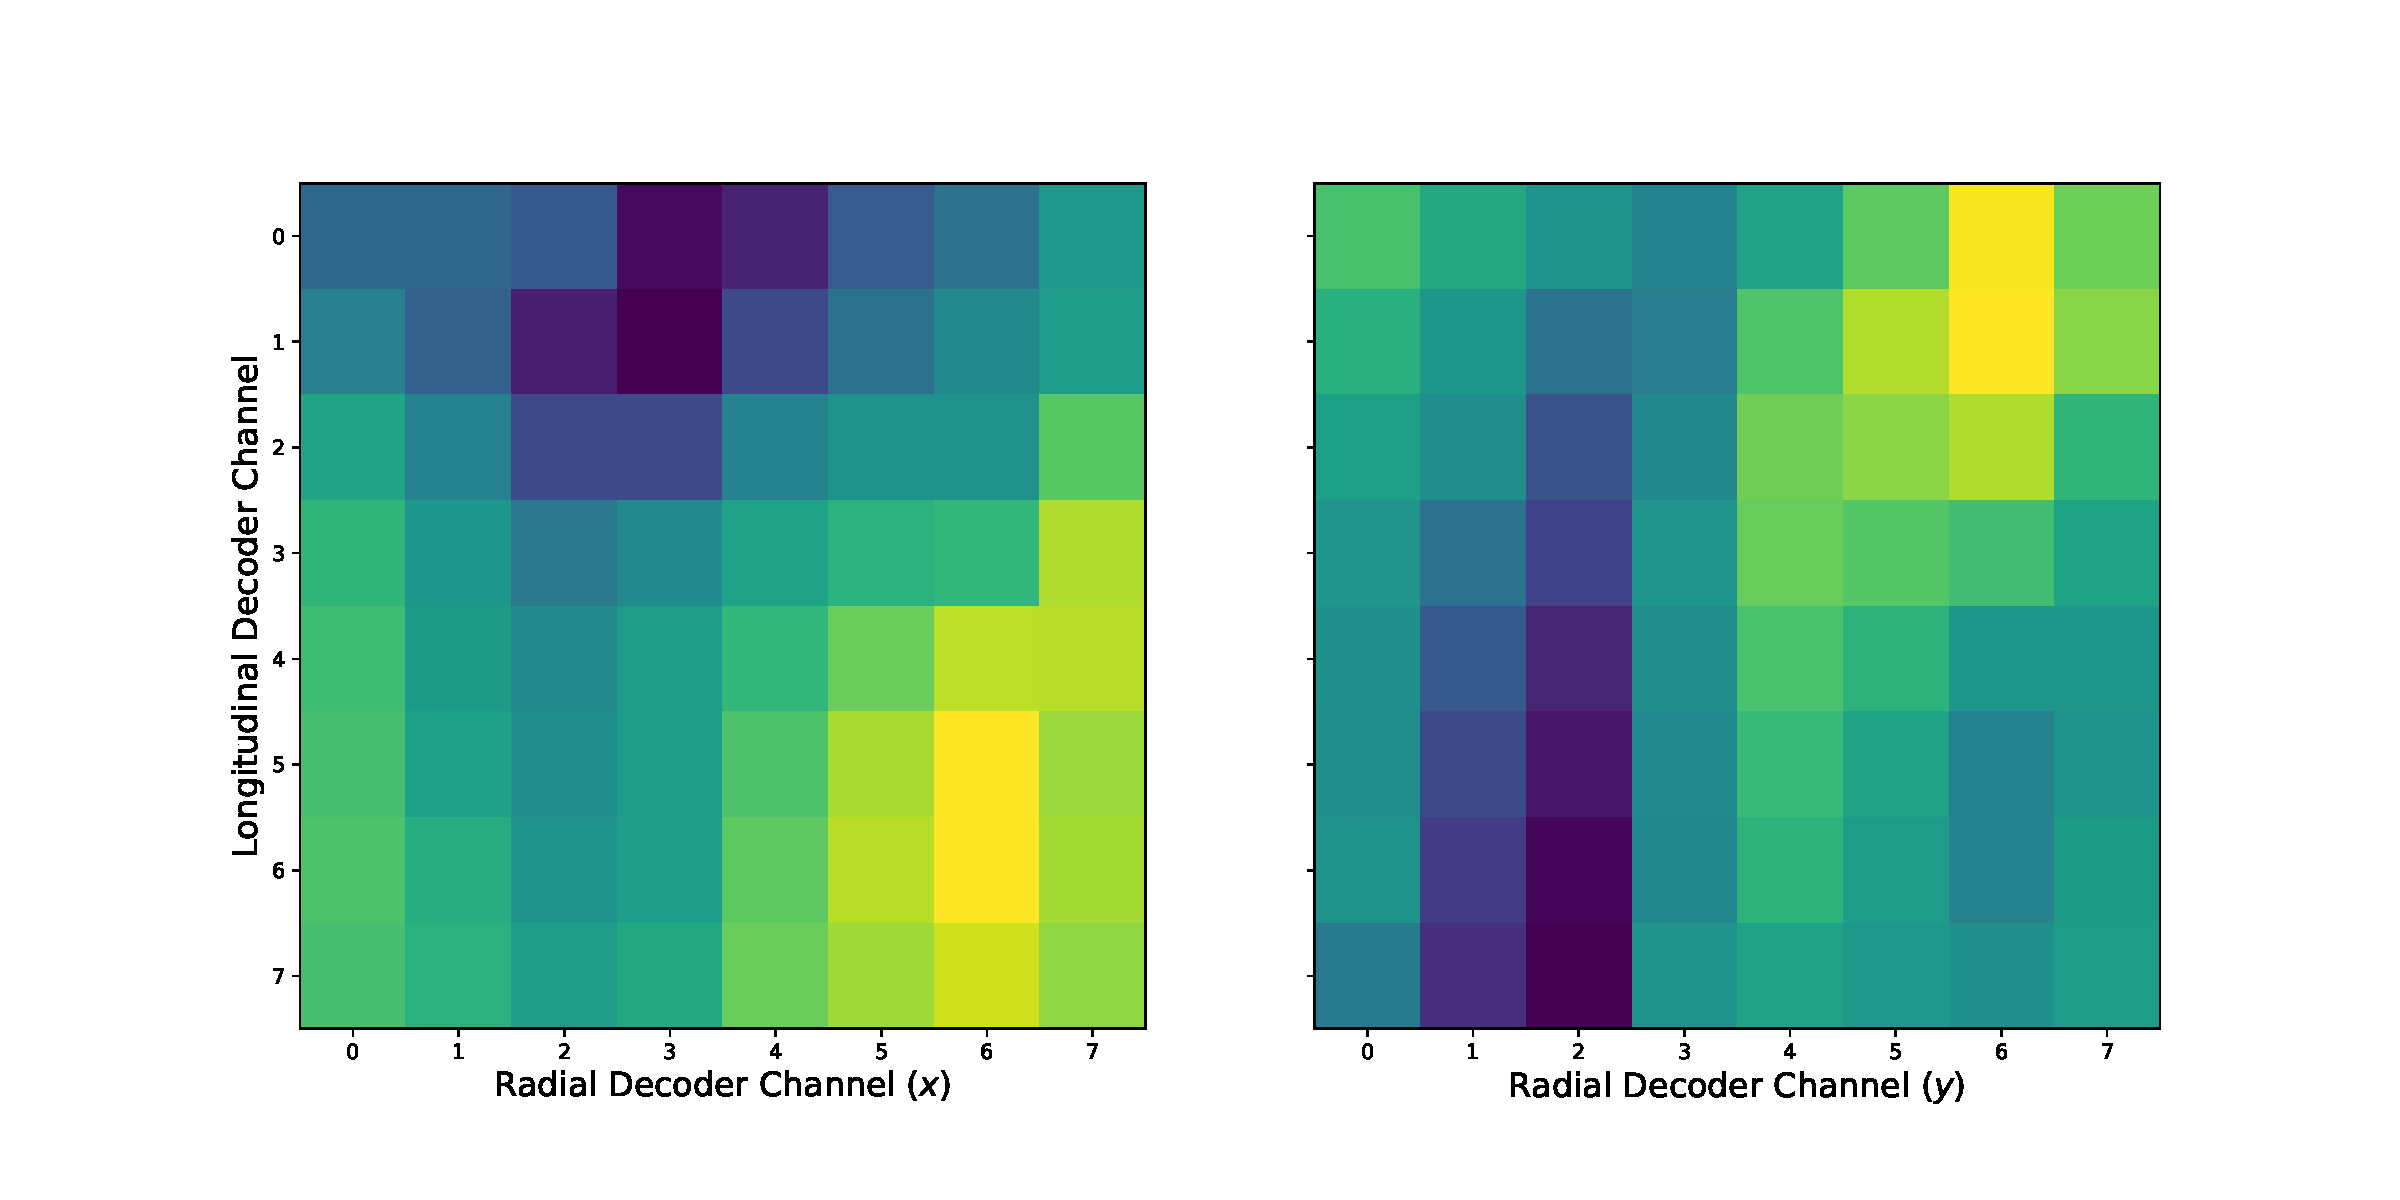
\includegraphics[width=\textwidth]{analysis/decoder_heatmap.pdf}
\caption{Example EMG-to-force decoders from a single subject. The
``center hold, reach out'' task works by mapping 64 channels of EMG
activity from subjects' forearms to a 2-dimensional force vector, a
component acting in the \(x\) and \(y\) directions within the task's
linear dynamics. Depicted here are the two 64-dimensional ``decoders''
arranged as the EMG electrodes were arranged on subjects' arms (along
the arm, longitudinally, and around the arm, radially). The left plot
shows the \(x\) force decoder, and the right plot the
\(y\).}\label{fig:decoders}
\end{figure}

\begin{figure}
\centering
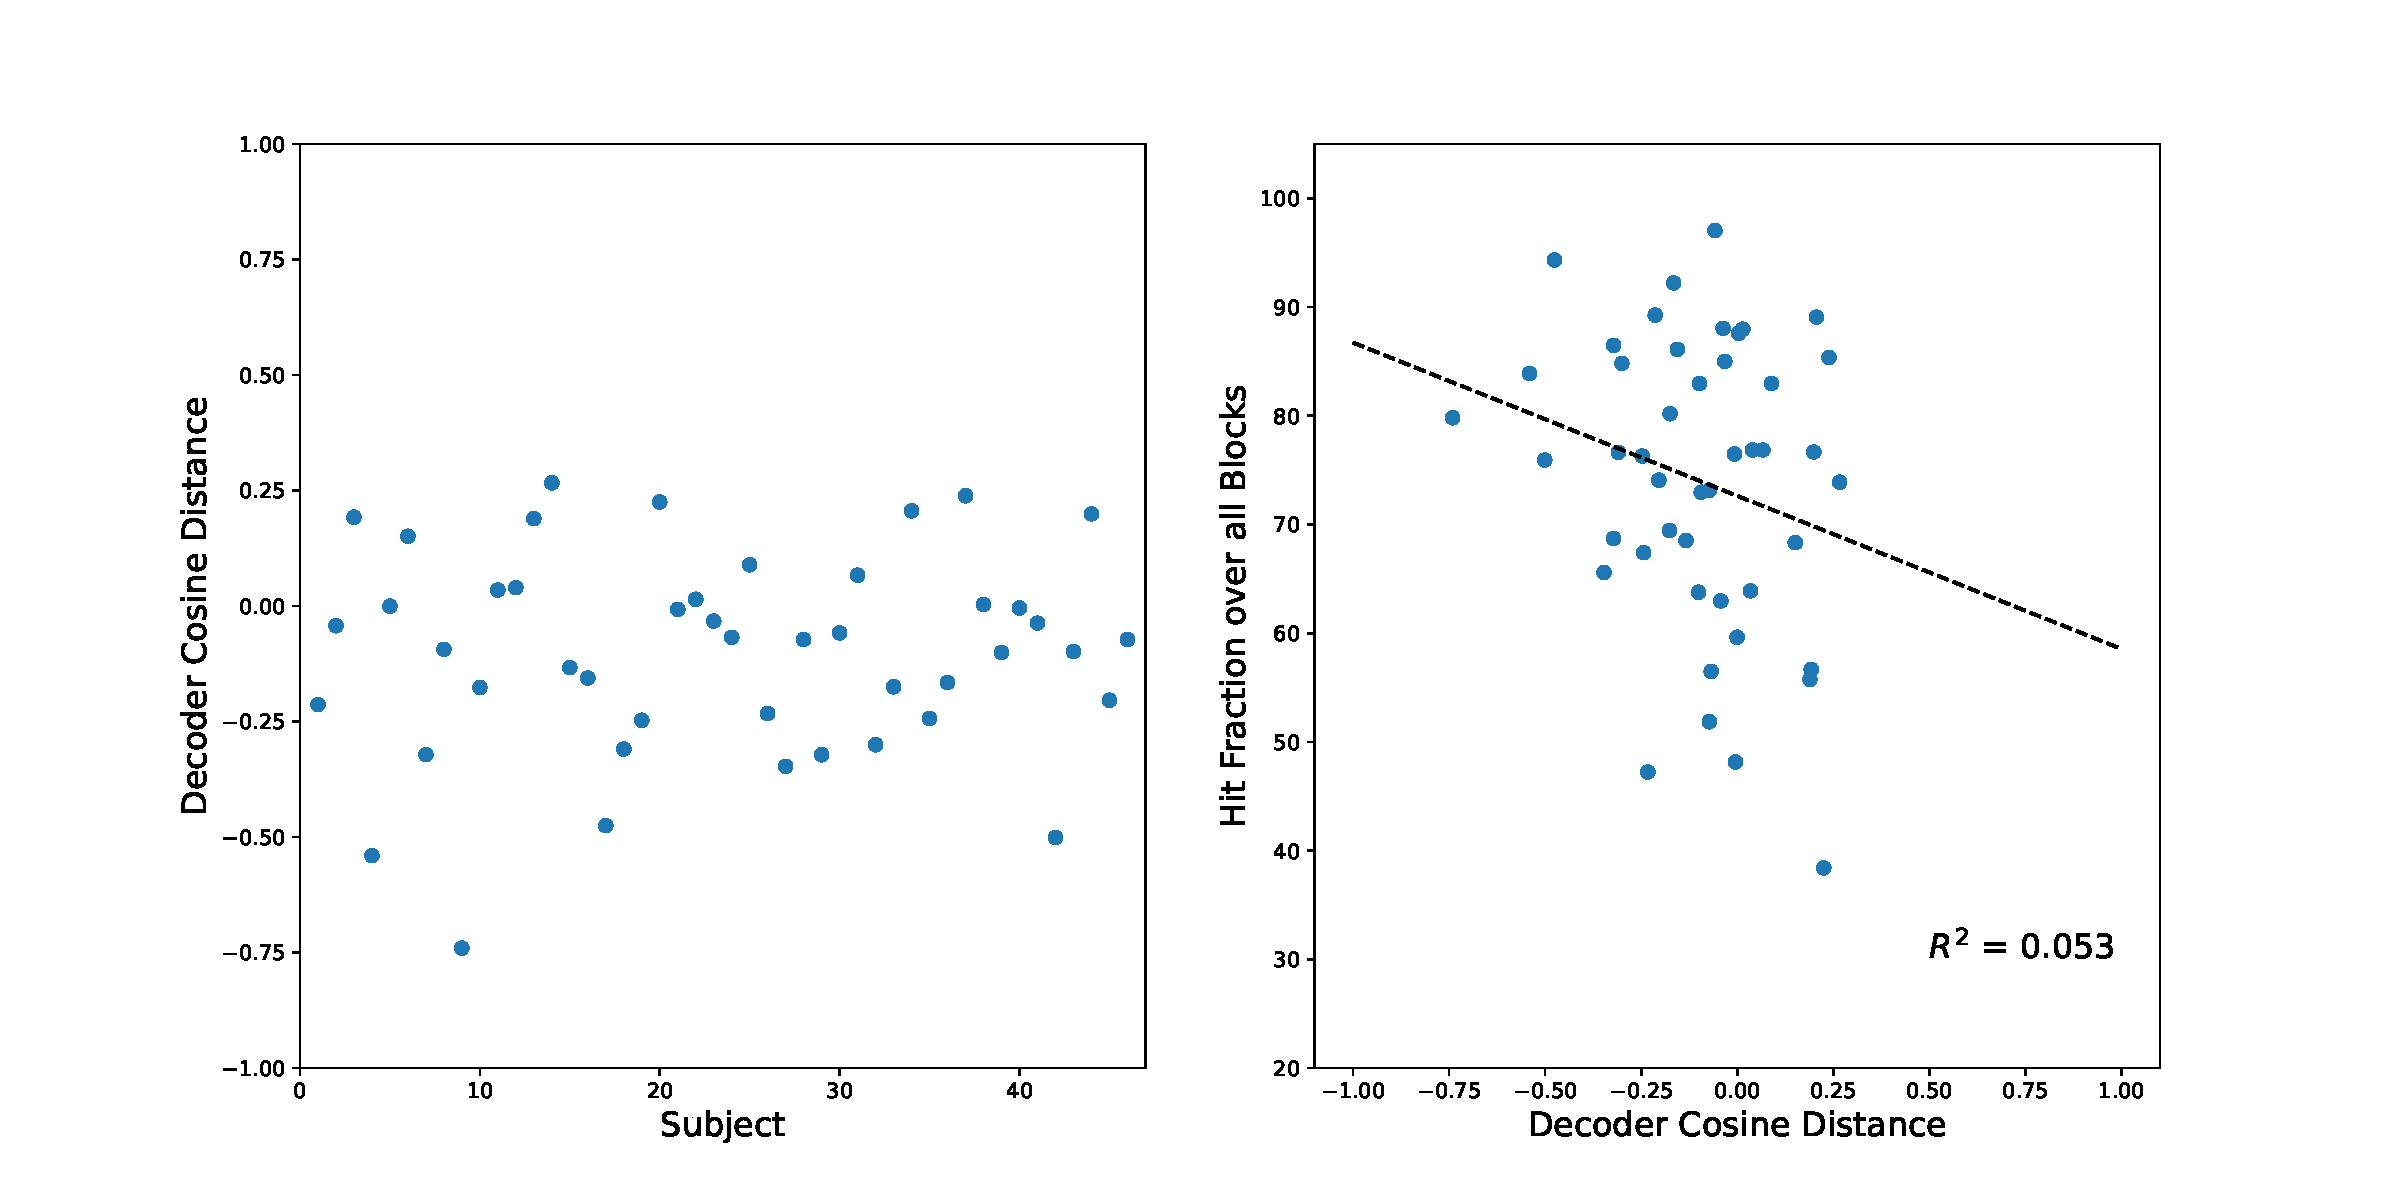
\includegraphics[width=\textwidth]{analysis/decoder_correlation.pdf}
\caption{Decoder cosine similarity. EMG-to-force decoders are computed
using a calibration dataset collected before the ``center hold, reach
out'' task. 4 ``modes'' of EMG activity are extracted from the dataset
using non-negative matrix factorization. These 4 modes are then
subtracted in pairs to yield the two 64-dimensional EMG-to-force
mappings, shown in \{+@fig:low\_variance\_PCs\}. The left plot shows the
cosine similarity of the \(x\) and \(y\) EMG-to-force decoders. A cosine
similarity of 1 means the two vectors are parallel, producing identical
forces (in the respective directions) for the same EMG activity
(\(F_x = F_y\)). A cosine similarity of -1 means the vectors are
antiparallel, producing equal but opposite forces in the two directions
(\(F_x = -F_y\)). A cosine similarity of 0 means the decoder directions
are orthogonal; e.g.~producing a force in the \(x\) direction with a
certain EMG activity produces no force in the \(y\) direction. Plotted
across subjects, we see a range of decoder similarities, providing a
variety of task contingencies. The rightmost plot asks whether cosine
similarity is predictive of task success, in terms of the numbers of
``Hits''. We find no significant correlation, implying that the decoder
cosine similarity, in the range we tested, does not predict task
success. Task success, therefore, likely relies on an alternative task
variable.}\label{fig:decoder_correlations}
\end{figure}

\begin{figure}
\centering
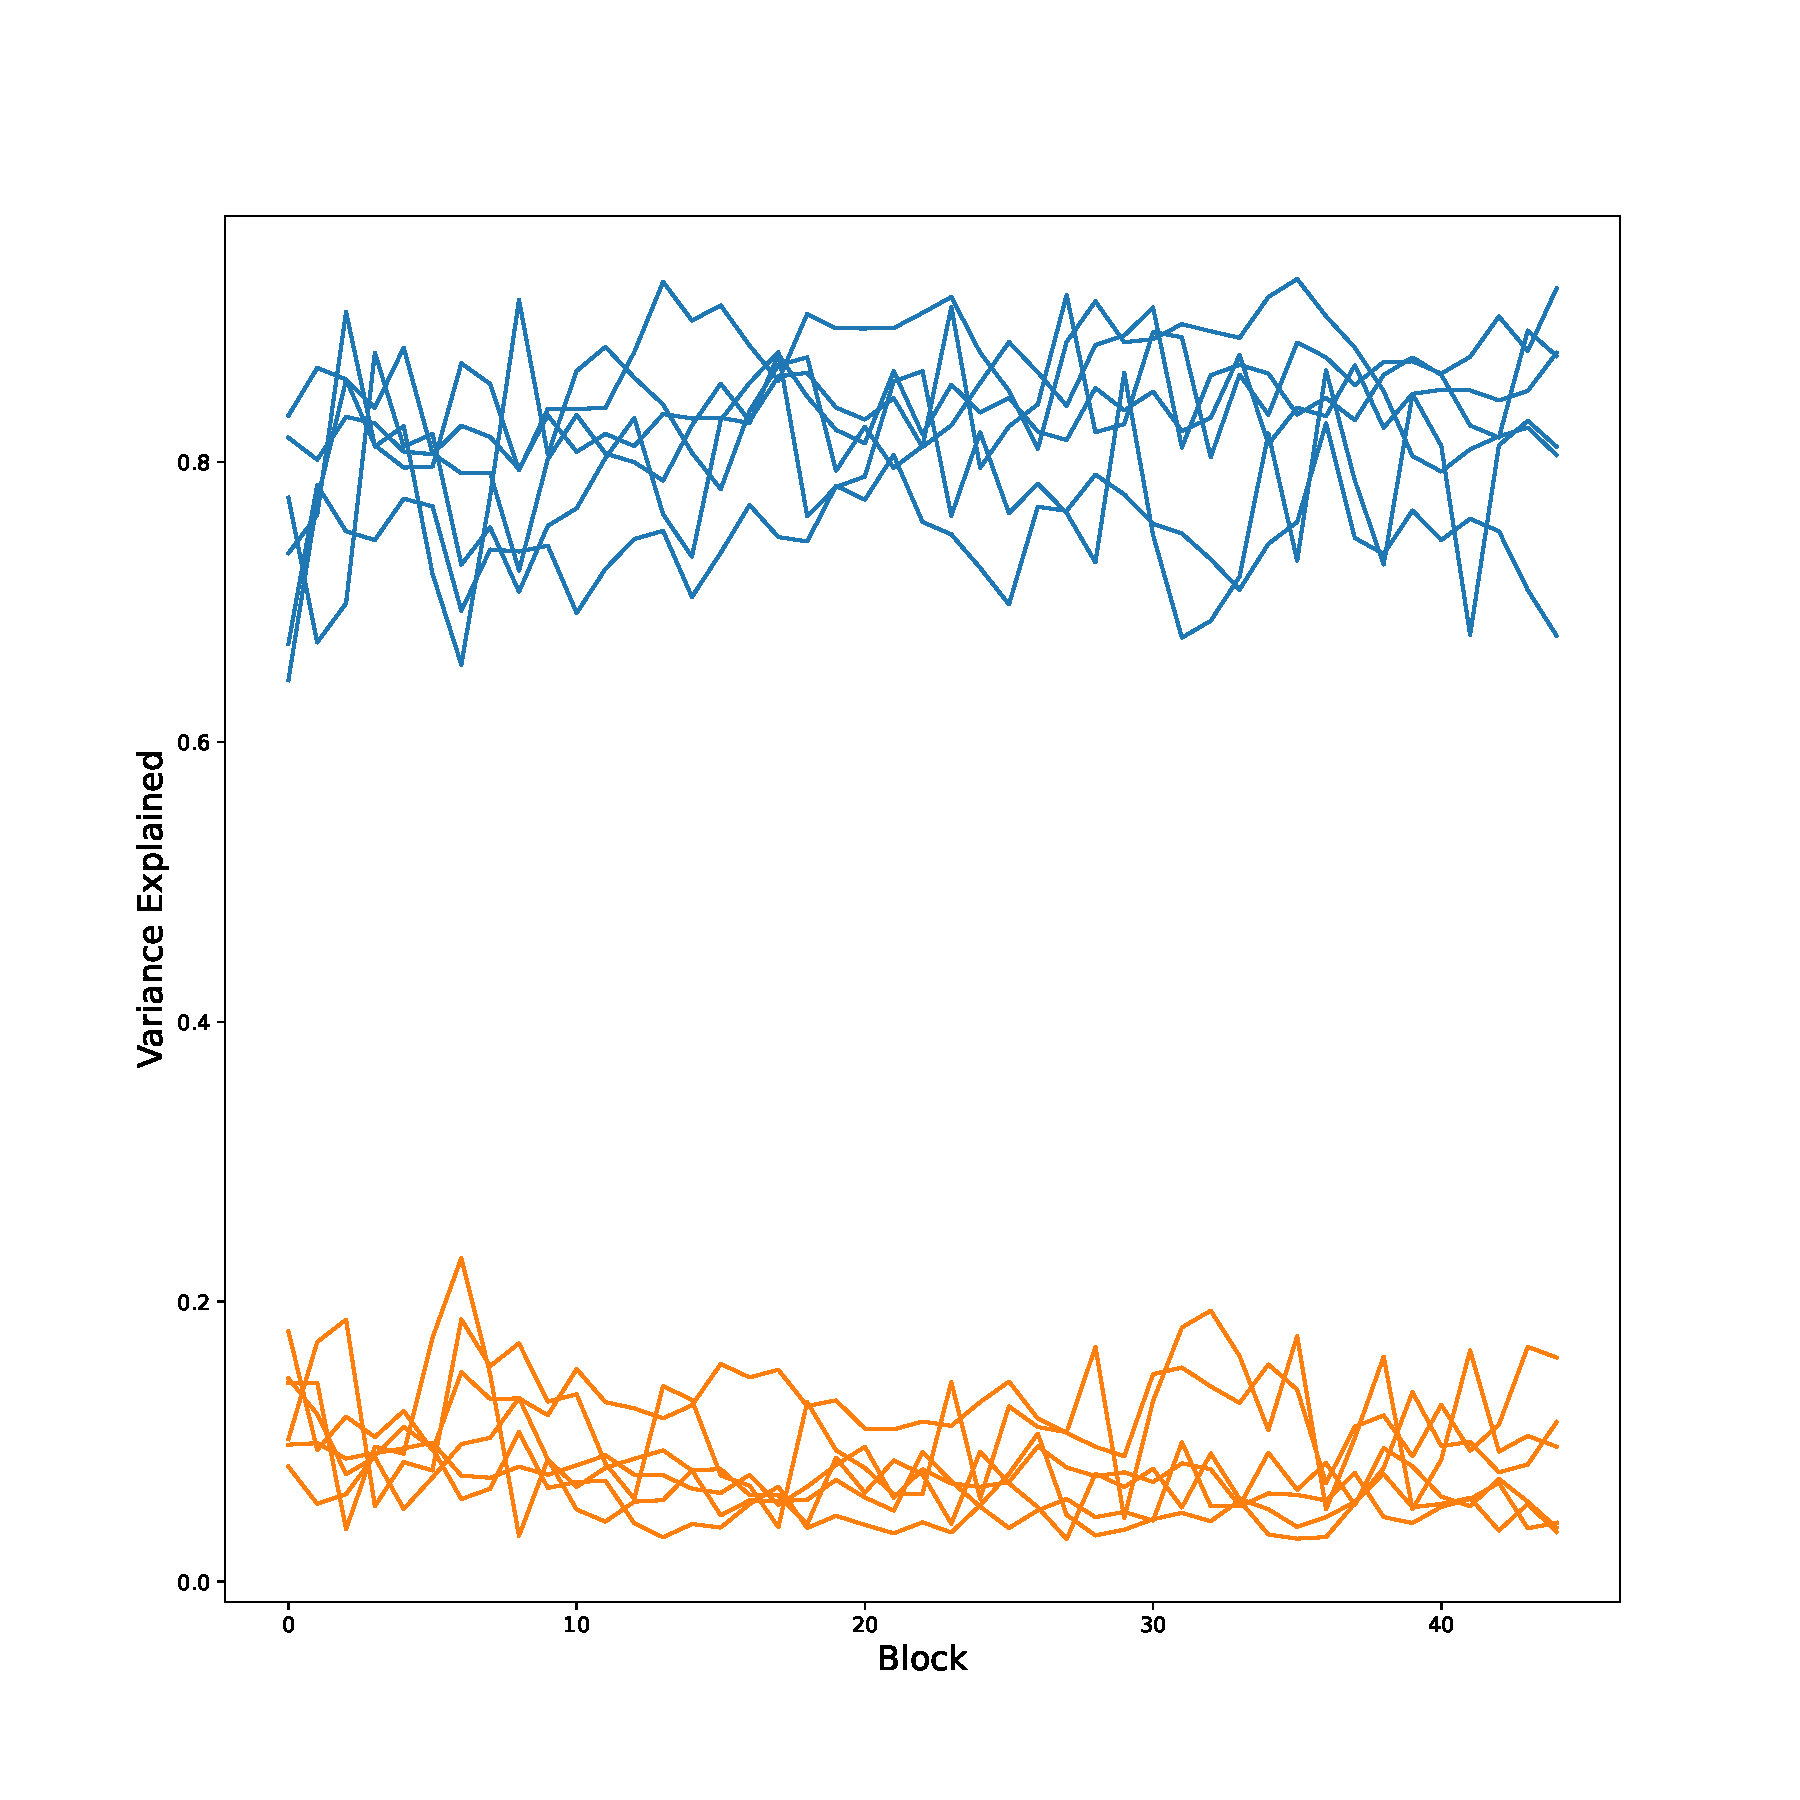
\includegraphics[width=\textwidth]{analysis/PCA_blocks.pdf}
\caption{PCA of EMG activity over blocks. The experimental paradigm is
unique in that we have access to the true subject state (EMG activity),
control over the contingency (the decoding from EMG to force in the
task), and the outcome (task behavior). This plot addresses the question
of whether there is a dynamic, over blocks, of the variance of the EMG
signals concatenate over blocks (12 trials). The plot suggests this is
not the case, as the first PCA component of EMG activity, for six
subjects, explains much of the EMG variance for each block, without any
visual indiciation of a trend. This is a common finding, and confirms
what is often found in the literature, that joint and/or muscle
activity, while high-dimensional, displays low dimensional modes.
Exploring the structure of the variance of this signal is a next step,
to understand how subjects manage the variability of their activity to
acheive task success, and how this evolves over
trials.}\label{fig:behavior}
\end{figure}

\newpage

\cref{fig:outcomes}
\cref{fig:decoders}
\cref{fig:decoder_correlations}
\cref{fig:behavior}

\end{document}